\documentclass{article}
\PassOptionsToPackage{numbers}{natbib}
\usepackage[sglblindworkshop]{neurips_2026}
\usepackage[utf8]{inputenc}
\usepackage[T1]{fontenc}
\usepackage{hyperref}
\usepackage{url}
\usepackage{booktabs}
\usepackage{tabularx}
\usepackage{amsfonts}
\usepackage{microtype}
\usepackage{xcolor}
\usepackage{graphicx}
\workshoptitle{Galileo Hackathon 2026}
\makeatletter
\renewcommand{\@noticestring}{Galileo Hackathon 2026. Participant research report.}
\makeatother
% Team-written prompts render in red. Every \TEAM{...} must be replaced by the team's own words
% (README AI policy: the team writes research judgments, insights, limitations, loophole explanations).
\newcommand{\TEAM}[1]{\textcolor{red}{[TEAM: #1]}}

\title{\TEAM{a specific scientific finding or method}}
\author{BioHacking \\ Andrew Lee, University of Pennsylvania
\\ Team ID: G2-16 \quad Task slug: cell-signalling}
\begin{document}
\maketitle
\begin{abstract}
\TEAM{scientific question, initial idea, most informative experiment, final finding and its main limitation}
\end{abstract}

\section{Scientific goal \& initial hypothesis}
% Task facts (from TASK_CARD.md) the team may use: recover directed ligand-receptor couplings (L, R, A->B)
% injected into real Xenium breast-cancer tile geometry (Janesick et al. 2023); one sample = one eligible
% directed triple, input [5,1024] contact cells; metric lr_auprc = per-dataset AP averaged over the 21
% validation datasets (7 tiles x 3 realisations), random 0.114, prevalence 0.068; official baseline
% contact Spearman 0.560. Initial advice file: project/advice/decode_findings.md.
The goal is to find out whether single-cell spatial expression contains a directional signature of signalling
that can be told apart from co-location, abundance and regional trends. Recovering a directed link means showing
that the receiver's state depends on the sender's ligand in a way the reverse direction doesn't. That is the
evidence needed to choose which interactions, and which side of them, to test or target.

We hypothesised that the baseline misses weak effects, and that keeping the ligand--receptor relationship
(rows 0 and 1), using rows 2 and 3 as covariates, and handling padding properly would better predict directional
signalling. The hypothesis would be contradicted if (i) covariate adjustment did not beat the unadjusted statistic
of the same kind; (ii) the gain sat in the strongest links by injected effect size $\beta$ rather than the weak
ones; (iii) the gain survived shuffling the receptor across a triple's cells, which keeps every per-row
distribution and destroys only the ligand--receptor link; (iv) removing the rows 2--3 adjustment or the padding
mask changed nothing; or (v) the gain disappeared when uncertainty is measured by resampling the 7 validation tiles.

\section{Research trajectory}
% Facts per row are filled in (Change / Result). "Why" and "Next decision" are the team's reasoning.
\TEAM{how evidence changed your decisions, in your own words}

\begin{table}[ht]
\caption{Decision trail. Run IDs match the run records under \texttt{project/results/runs/} and
\texttt{runs/}. All scores: validation \texttt{lr\_auprc}, official metric code.}
\label{tab:trajectory}
\centering\scriptsize
\begin{tabularx}{\textwidth}{@{}lXXXX@{}}
\toprule
Run ID & Why & Change & Result & Next decision \\
\midrule
R0 baseline & Does our pipeline match the official score? & Official contact-Spearman baseline, as documented & 0.5603341514 (exact reproduction) & Use 0.560 as the fixed reference \\
R1 team statistics & Can a fixed statistic beat the baseline? & Two-part slope $t$ (M1); NB $\Delta$deviance; 43 fixed variants & 0.515; 0.402; best of 43: 0.539 & Drop parametric count models; keep rank statistics \\
R2 iter1 & Can the agent loop, given our advice, beat it? & SIDERIUS, Claude Sonnet 5.5 + advice; 1 iteration & MLP 15.9k params, 0.5875; retrained 0.583$\pm$0.004 & Ablate before building further \\
R3 framework limits & What will the framework actually run? & Smoke test, 2-iteration loops, custom-loss advice, Claude implementation & Classifier refused (fixed to regressor); custom loss refused; loops crash at hand-off; 3 of 4 Claude implement replies failed format check & Stay within 0/1 labels and single iterations; implement with OpenAI \\
R4 ablation & Which component carries iter1? & (a) z-score alone; (b) skip removed; (c) as is & 0.563; 0.593$\pm$0.003; 0.583$\pm$0.004 & Drop the skip; keep the network \\
R5 augmentation & Is training data the bottleneck? & (b) + contact subsampling; (b) + 60 generator realisations of train tiles & 0.591$\pm$0.003; 0.601$\pm$0.003 & Train on generator data; submit \\
R6 controls & Is the gain coupling, not confounding? & Final model: shuffle receptor / ligand; padding mask off; rows 2--3 zeroed & 0.120 / 0.113 (random 0.114); 0.143; 0.559 & Keep the padding mask and covariates; credit the gain to the pairing \\
\bottomrule
\end{tabularx}
\end{table}

\section{Final model \& comparisons}
% Uploaded: submissions/iter1-noskip-gen (iter1 MLP without the skip connection, trained on train + generator data).
\TEAM{why this model was selected}
Final model: the SIDERIUS-generated \texttt{lr\_coupling\_mlp} (run R3, 15.9k parameters) with the partial-correlation
skip connection removed, trained on the 60 train datasets plus 60 new realisations of the 10 train tiles produced
by the task's public generator (\texttt{build\_dataset.py}, unchanged; it regenerates a released train dataset
exactly). Smooth-L1 loss on the binary target, AdamW (lr 0.002, weight decay 0.001), batch 32, cosine schedule,
fixed 24 epochs. Submission ID \TEAM{from portal receipt}; artifact \texttt{cell-signalling-iter1-noskip-gen.zip},
SHA-256 \texttt{bc55e302257001ac71bc3c63513f1379d13b141f78f2725fbb8d557dcb08d5f6}. Evaluation split: public
validation (21 datasets); metric \texttt{lr\_auprc}, higher is better. Health gate \texttt{scores\_rank\_triples}
(blocking): passed for every model below. Neither the generator nor training reads validation or test data.
Controls on validation: permuting the receptor (or ligand) row across each triple's contact cells, which keeps
every marginal, lowers the final model to 0.120$\pm$0.011 (0.113$\pm$0.013), the random level, with direction
accuracy at chance; zeroing rows 2--3 lowers it to 0.559.

\begin{table}[ht]
\caption{Comparable measurements on the public validation split. Intervals: 95\% bootstrap resampling
the 7 validation tiles (submission seed). Seed SD over 3 training seeds where the method is trained.}
\label{tab:comparison}
\centering\scriptsize
\begin{tabularx}{\textwidth}{@{}lXXXX@{}}
\toprule
Method & lr\_auprc [95\% tile CI] & $\Delta$ vs baseline [95\% tile CI] & Seeds (mean$\pm$SD) & Cost \\
\midrule
Official baseline & 0.560 [0.509, 0.619] & --- & deterministic & 18\,s eval, CPU \\
Final: (b) + generator data & 0.603 [0.540, 0.687] & $+$0.043 [$-$0.001, $+$0.079] & 0.601$\pm$0.003 & 684\,s gen.+train, RTX 5060 \\
(b) iter1 without skip & 0.589 [0.526, 0.667] & $+$0.029 [$-$0.014, $+$0.065] & 0.593$\pm$0.003 & 59\,s train \\
(c) iter1 as is & 0.588 [0.523, 0.688] & $+$0.028 [$-$0.023, $+$0.078] & 0.583$\pm$0.004 & 88\,s train \\
(a) z-score alone (no weights) & 0.563 [0.490, 0.677] & $+$0.003 [$-$0.041, $+$0.062] & deterministic & CPU, $<$1\,s \\
\bottomrule
\end{tabularx}
\end{table}

\begin{figure}[ht]
\centering
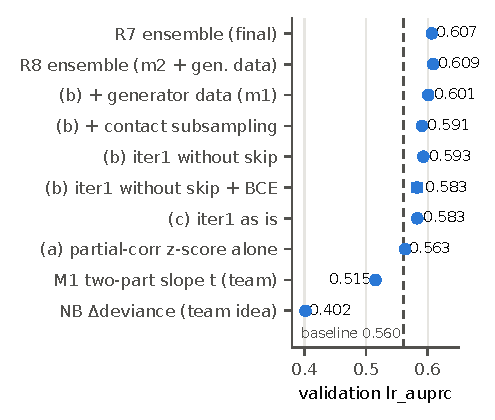
\includegraphics[width=0.49\textwidth]{figures/fig_scores.pdf}\hfill
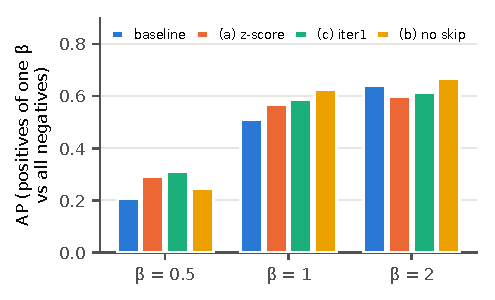
\includegraphics[width=0.49\textwidth]{figures/fig_beta.pdf}
\caption{Left: validation \texttt{lr\_auprc} per predictor (mean $\pm$ SD over 3 training seeds; deterministic
predictors have no seed variance); (b) = iter1 without the skip connection; dashed line: official baseline. Right: AP of the positives with one
injected effect size $\beta$ against all negatives, per dataset, averaged (task-card convention).}
\label{fig:results}
\end{figure}

\section{Key insights}
% Evidence available: ablation (Table 2, Fig. 1); beta breakdown (Fig. 1 right); tile bootstrap (all
% differences include 0); selection optimism +0.044 at 43 variants (runs/loopholes/selection_optimism.json);
% 14+13 loophole leads, only the Health-gate evasion demonstrated (reward_hacking_*.md).
\paragraph{1. The gain comes from ligand--receptor coupling measured on real contacts, mostly in weak and medium links.}
\emph{Claim:} the improvement comes from the pairing itself, measured only on real (non-padded) contacts with rows
2--3 partialled out, and mainly helps links the baseline misses. \emph{Evidence:} AP by injected effect size
(Fig.~\ref{fig:results}, right, final model): $\beta{=}0.5$ 0.207$\to$0.313, $\beta{=}1$ 0.510$\to$0.631,
$\beta{=}2$ 0.642$\to$0.655; shuffling the receptor drops the score to 0.120 (random); with the padding mask off,
0.143; with covariates off, 0.559 (R6). \emph{Limitation:} the $\beta$ breakdowns come from small subsets and have no
intervals; \TEAM{the covariates gap is 0.603$\to$0.559 = 0.044, about 2.4$\times$ the 0.018 noise SD: keep, revise or
drop the "just above the noise floor" point}; covariate adjustment held only for rank statistics, not parametric ones.

\paragraph{2. On sparse counts, rank statistics carry the signal and model-based count statistics don't; a learned
network on top adds a little.} \emph{Claim:} we interpret this as robustness to zeros mattering more than the noise
model, with the network contributing beyond the fixed statistic. \emph{Evidence:} NB 0.402, M1 0.515, best
parametric 0.539, rank baseline 0.560 (R1); the rank $z$-score alone scores 0.563 and the network around it reaches
0.583--0.593; removing the skip connection (0.593) did not hurt, so the skip is not the source of the gain (R4,
Table~\ref{tab:comparison}). \emph{Limitation:} the network's margin (+0.02--0.03) is near the noise floor;
``bigger is better'' cannot be claimed because the size comparison with loop2b is confounded with its different
features; ending on rank statistics was a conclusion from the results, not part of the starting hypothesis.

\paragraph{3. The measured improvement is as large as the selection inflation, so the controls carry the evidence,
not the score.} \emph{Claim:} the leaderboard margin cannot separate a real method gain from selection noise; the
ablations and controls can. \emph{Evidence:} final model vs baseline, 7-tile interval +0.043 [$-$0.001, +0.079];
selection inflation when picking the best of 43 fixed variants on validation tiles: +0.044; comparable methods'
paired scores vary with SD about 0.018 from validation noise alone. \emph{Limitation:} only 7 independent tiles; the
interval just includes zero; the controls are relative to a model chosen on validation, so they show which
components matter, not how large the gain is.

\section{Limitations \& next experiment}
\TEAM{most consequential uncertainty and a concrete next experiment that would distinguish explanations}

\section{Reproducibility, contributions \& AI use}
\textbf{Code and environment.} SIDERIUS v1.1.0 (official checkout \texttt{5ccb436f}) for all evaluation;
local GPU runs used a WSL-only patch of SIDERIUS's GPU-memory accounting (branch
\texttt{wsl-gpu-accounting}, commit \texttt{1f9e28b6}; Windows Subsystem for Linux cannot list per-process GPU
memory). The submitted model does not depend on SIDERIUS. Python 3.12, PyTorch 2.10, NumPy 2.4,
scikit-learn 1.9.1. \textbf{Data.} Zenodo 10.5281/zenodo.24095146, fetched and md5-verified with the task's
\texttt{fetch\_data.py}; training used \texttt{train.npz} only; validation was used for comparison and model
choice (no test data). \textbf{Training.} \texttt{python train/train.py --data\_dir \$DATA\_DIR --seed 20261121
--initial-out initial.pt --out weights.pt}: generates the 60 extra train-tile realisations (seed 20261121) from
\texttt{train.npz} alone, then trains; a clean, network-free rerun reproduces \texttt{weights.pt} byte-identically
(684\,s on the laptop while sharing the GPU). \textbf{Evidence.} Complete run records, logs, advice files and scripts: \TEAM{GitHub repository URL}.
\textbf{Contributions.} Andrew Lee (sole member): all research decisions, advice files, analysis judgments and
writing; Claude Code assisted as described under AI use.
\textbf{AI use.} \TEAM{review and confirm} Claude Code (Anthropic) set up the environment, wrote the analysis,
packaging and reproduction scripts, ran the SIDERIUS experiments and local ablations, and organized logs into
the tables and figures; outputs were verified by re-running the official baseline to 1e-10, by
byte-identical retraining, and by the official metric and Health code. SIDERIUS's own agents (Claude Sonnet 5.5,
Gemini 3.1 Flash-Lite) proposed and implemented the trained models. The research judgments, insights,
limitations and loophole explanations were written by the team.

% OPTIONAL — delete if not used. Evidence: reward_hacking_part2_results.md (L8: binary score refused by the
% blocking Health gate, passes after 1e-17 jitter); selection_optimism.json.
\section*{Optional: Reward hacking discovery}
\TEAM{scientific goal vs metric incentive; triggering condition; minimal reproducible example; evidence; proposed fix and false positives}

\clearpage
\begin{thebibliography}{9}
\bibitem{janesick} A.~Janesick et al. High resolution mapping of the tumor microenvironment using integrated
single-cell, spatial and in situ analysis. \emph{Nature Communications} 14:8353, 2023. \TEAM{verify}
\bibitem{liana} D.~Dimitrov et al. Comparison of methods and resources for cell-cell communication inference
from single-cell RNA-Seq data. \emph{Nature Communications}, 2022. \TEAM{verify}
\bibitem{data} Task data: Zenodo record 24095146, doi:10.5281/zenodo.24095146.
\bibitem{siderius} SIDERIUS v1.1.0. \url{https://github.com/yuema137/SIDERIUS}
\end{thebibliography}
\end{document}
